\documentclass[11pt, oneside]{article}
\usepackage[margin=1in]{geometry}
\geometry{letterpaper}
\usepackage{booktabs}
\usepackage{hyperref}
\usepackage{enumitem}
\usepackage{float}
\usepackage{caption}
\usepackage{subcaption}
\usepackage[numbers]{natbib}
\usepackage{graphicx}
\usepackage{amssymb}
\usepackage{amsmath}
\usepackage{array}
\usepackage{longtable}
\usepackage{xcolor}
\usepackage{tabularx}
\usepackage{setspace}
\usepackage{tikz}
\usetikzlibrary{positioning,arrows.meta,fit}
\hypersetup{
    colorlinks=true,
    linkcolor=blue,
    citecolor=blue,
    urlcolor=blue
}
\captionsetup{font=small,labelfont=bf,skip=3pt}
\setlength{\textfloatsep}{8pt plus 2pt minus 2pt}
\setlength{\floatsep}{6pt plus 2pt minus 2pt}
\setlength{\intextsep}{6pt plus 2pt minus 2pt}
% ============================================================
% TITLE BLOCK --- students must keep this format
% Filename of the compiled PDF must be:
% CS781-CP-[Firstname]-[Lastname]-[RollNo]-report.pdf
% ============================================================
\title{CS781 Capstone Project:\\
In-House Legal Intelligence System}
\author{
    Suraj Singh Raman  \\
    261110067 \\
    {\tt ssraman26@iitk.ac.in}\\
    Indian Institute of Technology Kanpur (IIT Kanpur)
}
\date{}
\begin{document}
\maketitle
\begin{abstract}
A law firm needs to handle client information that must be kept confidential, and hence it should not use LLM APIs hosted externally by some third-party AI company.
This report describes a small legal language-model stack that a firm could host itself. With a byte-level BPE tokenizer trained on the course corpus, I pretrained four models of 54--62M parameters from scratch on 150M tokens of Indian acts, High Court, Supreme Court and tribunal judgments: three decoders (one without positional encoding, one with sliding-window attention and GQA, one with ALiBi and multi-head latent attention) and a bidirectional encoder--decoder. These checkpoints were fine-tuned to solve the six downstream tasks. The methods used for fine-tuning included partial, parameter-efficient fine-tuning and distilling a fine-tuned model into a 7-layer student. The encoder--decoder gave my best Phase-1 and Phase-2 submissions. The 36.6M student gave the best submissions in Phases 5--7 and scored above its own teacher in Phases 4 and 5. When the Phase-1 curves are plotted against tokens rather than steps, the three decoders turn out to learn at nearly the same rate. Two runs failed, and I analyse why.
\end{abstract}

% ============================================================
\section{Competition Result}
% ============================================================
\noindent
\textbf{Codabench username:} \texttt{s\_261110067}
\hfill
\textbf{Roll number:} 261110067

\begin{table}[H]
\centering
\small
\caption{Official phase scores and ranks (best valid submission per phase).}
\label{tab:leaderboard}
\begin{tabular}{clccc}
\toprule
Phase & Task & Primary metric (value) & Rank & Valid submissions \\
\midrule
1 & Legal LM Pretraining & BERTScore F1 = 0.8358 & 28 & 7 \\
2 & Legal NER & Strict macro-F1 = 0.3729 & 110 & 7 \\
3 & Rhetorical role prediction & Macro-F1 = 0.4380 & 102 & 4 \\
4 & Court judgment prediction & Macro-F1 = 0.7249 & 67 & 5 \\
5 & Legal statute identification & Macro-F1 = 0.4399 & 12 & 5 \\
6 & Abstractive summarization & BERTScore F1 = 0.8512 & 19 & 4 \\
7 & Prior Case Retrieval (PCR) & Micro-F1@7 = 0.4389 & 42 & 7 \\
\bottomrule
\end{tabular}
\end{table}

\noindent
\textbf{Total valid Codabench submissions across all phases:} 39
\quad
\textbf{Date ranks were recorded:} 9 November 2026

\smallskip
\noindent Every phase meets the minimum of four distinct submissions. The seven Phase-1 submissions come from four architectures (five checkpoints): Dec-02 contributed three decoding variants of one checkpoint, and the encoder--decoder was submitted before and after a bug fix. Two Phase-2 submissions are re-runs of a configuration after I added the distillation export. Code, notebooks with all outputs, and every submission file are at \url{https://github.com/ascyrax/legal-lm-from-scratch}.

% ============================================================
\section{Introduction and Problem Description}
% ============================================================
Legal documents often cannot leave the firm, so the realistic alternative to hosted LLMs is a small model the firm trains and serves itself. The capstone asks what such a model can do when built from nothing: no pretrained weights, no external corpora, 50--300M parameters, and free Kaggle GPUs (one T4, about nine hours per session).

Phase~1 continues a 512-word judgment prefix by 128 words (BERTScore F1~\cite{zhang2020bertscore}, with ROUGE-L~\cite{lin2004rouge} and BLEU-4~\cite{papineni2002bleu}). Phase~2 (L-NER) marks character spans of twelve entity types under strict span macro-F1; Phase~3 assigns one of thirteen rhetorical roles to each sentence in Corporate Law (CL) and IT judgments; Phase~4 (CJPE) predicts the binary outcome of an appeal; Phase~5 (LSI) assigns a set of statutes out of 100 (all three macro-F1). Phase~6 summarizes a judgment (BERTScore F1, ROUGE-1/L), and Phase~7 (PCR) returns exactly seven cited prior cases per query (micro-F1@7).

The questions I kept coming back to were practical ones. At about 55M parameters and one GPU, is any change to standard attention worth making? A 1,024-token model has to read judgments several times that long, so what should it read? And how much of a task can be learned by touching only a few million weights, or handed down from a larger fine-tuned model to a smaller one? Everything is implemented from scratch on top of plain PyTorch tensors: tokenizer, models, training loops, adapters, decoding and evaluation. I did not attempt instruction tuning, retrieval-augmented generation or ensembling, and I did not pipeline phases; every phase is a separate fine-tune of a Phase-1 checkpoint.

% ============================================================
\section{Data Analysis and Preprocessing}
% ============================================================
\subsection{Sources and official splits}
Only the official \texttt{Exploration-Lab/CS-781-Capstone} data were used (Table~\ref{tab:data}). Without a dev set, Phase~2 trains on fold~1 and validates on fold~2, and Phase~6 holds out 200 documents by hashing their IDs, with a checksum asserted in every notebook.

\begin{table}[t]
\centering
\footnotesize
\caption{Official splits and the statistics that informed design (token counts use my BPE tokenizer).}
\label{tab:data}
\begin{tabular}{p{0.5cm}p{3.6cm}p{10.3cm}}
\toprule
Ph. & Splits & Statistics that mattered \\
\midrule
1 & 4 sources; 150M / 0.7M tokens & High Courts: 65M tokens in 112,740 short documents; Supreme Court: 25M in 3,650 long ones; Acts 20M; Tribunals 40M. Final val loss ranges from 0.98 (High Courts) to 2.54 (Supreme Court). \\
2 & 2 folds $\times$ 35 docs; test 35 & 8,393 gold entities; DATE (813 in fold 1) and PREC (624) dominate, WIT (67) and A.COUNSEL (70) are rare; all offsets use an exclusive end. \\
3 & CL / IT: 40+40 train, 5+5 dev, 5+5 test & 10,593 CL and 6,252 IT training sentences; label mix differs by domain (Fig.~\ref{fig:data}a); \emph{Issue} has 17 CL examples, \emph{Dissent} occurs only in CL. \\
4 & 37,387 / 1,988 / 1,517 cases & Train 59\% class 0, dev exactly balanced. Median case 2,752 tokens (p90 6,928); a $4\times511$-token budget covers the whole case for only 38\%. \\
5 & 42,750 / 10,181 / 13,019 docs & 100 statutes, 3.7 per document; explicit section numbers appear in under 2\% of documents, but \texttt{<SECTION>}/\texttt{<ACT>} placeholders mark citation sites in 89\%. \\
6 & 7,030 pairs (6,830/200 local); 100 test & Median document 3.8k tokens, median summary 739; 1\% of pairs fit in 1,024 tokens. Summaries are extractive (fragment coverage 0.96, density 14.7~\cite{grusky2018newsroom}) and follow document order in 77\% of consecutive sentences. \\
7 & 827/118/237 queries; pools 4,320/1,023/1,727 & 5,308 train gold pairs; every query sits in its own pool; \texttt{<CITATION>} appears in 99.9\% of queries; the best achievable dev F1@7 is 0.618, since 59\% of queries have fewer than seven gold cases. \\
\bottomrule
\end{tabular}
\end{table}

\subsection{Corpus statistics that actually informed design}
High Court documents are short and formulaic (their validation loss is less than half that of Supreme Court text), so I sampled sources in proportion to token counts instead of up-weighting any. Phase-4 lengths make truncation unavoidable, so the question is \emph{which} 2,044 tokens to read; I read the last four chunks, where the operative order sits. In Phase~5 masking turns string matching into inference from facts, but placeholders still mark citation sites, so long documents keep the text around them. In Phase~6 extractiveness and document order suggested chunk-by-chunk summarization, and the U-shaped position of summary content (14\% of aligned sentences in the last decile, 7\% mid-document) argued against reading only the beginning.

\begin{figure}[t]
\centering
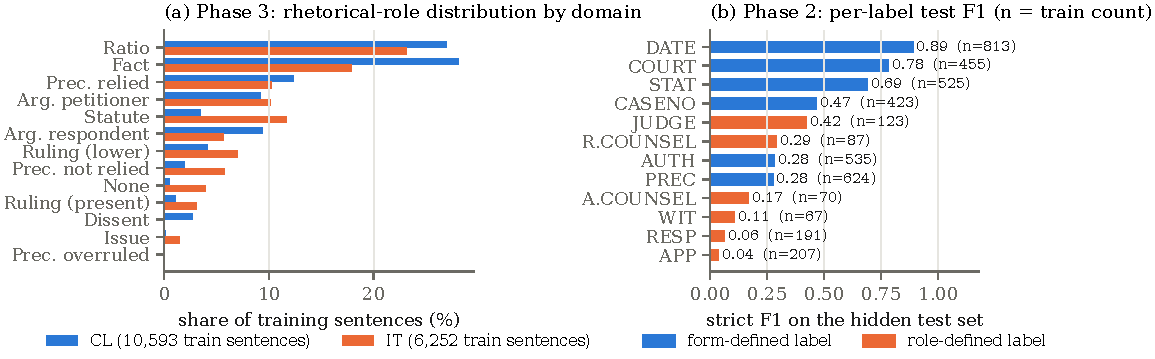
\includegraphics[width=0.80\linewidth]{figures/fig_data_ner.pdf}
\caption{(a) Rhetorical-role distribution in the two Phase-3 domains: IT cites statutes three times as often and has far more \emph{None} sentences. (b) Per-label strict F1 of my best Phase-2 submission on the hidden test set, with each label's training count. Labels defined by surface form are learned; labels defined by a party's role are not, regardless of frequency.}
\label{fig:data}
\end{figure}

\subsection{Preprocessing}
\textbf{Tokenizer.} I trained a byte-level BPE~\cite{sennrich2016bpe} with 32,000 entries on the Phase-1 corpora using only the Python standard library. Byte-level coverage removes unknown tokens, digits are split, and there is no normalization, which would shift Phase-2 offsets (1.25--1.42 tokens per word). Pre-tokens are capped at 1,000 bytes because scanned judgments contain 100k-character runs of dashes.

\textbf{Offsets, sentences and chunks.} The tokenizer returns character offsets for every token. Gold spans become BIO tags and predictions map back through the offsets; an oracle round trip reproduces all 8,393 gold spans exactly. Phase~3 uses the provided sentence lists unchanged and packs consecutive sentences into windows of up to 800 tokens with 50\% overlap. Phases 4--6 use 512- or 1,024-token chunks. In Phase~7 candidates are up to 16 chunks of 512 tokens (86\% of all tokens), and queries use an \emph{evidence view}: the head of the judgment plus the sentences around each \texttt{<CITATION>} marker.

% ============================================================
\section{Approach and Model Evolution}
% ============================================================
\subsection{Phase-1 foundation model}
All backbones share one block: pre-norm RMSNorm~\cite{zhang2019rmsnorm}, SwiGLU~\cite{shazeer2020glu}, $d_\text{model}=512$, eight 64-dimensional heads, tied embeddings and residual projections initialized with standard deviation $0.02/\sqrt{2L}$ (Table~\ref{tab:arch}). A guard computes the parameter count (tied embedding counted once) and refuses to train outside 50--300M.

\begin{table}[t]
\centering
\footnotesize
\caption{Phase-1 backbones. Tokens seen are measured from logged throughput. The encoder--decoder's loss is a sequence-to-sequence loss on continuation tokens and is not directly comparable.}
\label{tab:arch}
\setlength{\tabcolsep}{3.4pt}
\begin{tabular}{lcccc}
\toprule
 & Dec-01 & Dec-02 & Dec-03 & Enc-Dec (v2) \\
\midrule
Layers & 12 & 12 & 13 & 6 enc + 6 dec \\
Attention & MHA 8/8 & GQA 8/2, window 256 in 9 layers & MLA, latent 128 & bidir.\ enc; causal dec + cross \\
Positions & none (NoPE) & RoPE & ALiBi & RoPE \\
Parameters & 54.9M & 54.9M & 53.9M & 61.5M (encoder 35.7M) \\
Tokens / step & 33k & 33k & 131k & 64 seqs of 768+256 \\
Steps / hours & 5,750 / 7.0 & 12,749 / 6.6 & 4,591 / 8.4 & 15,488 / 6.8 \\
Tokens seen & $\approx$190M (fp32) & 418M & $\approx$600M & -- \\
Best val loss & 2.117 & 1.944 & 1.885 & 1.959 \\
\bottomrule
\end{tabular}
\end{table}

\begin{figure}[t]
\centering
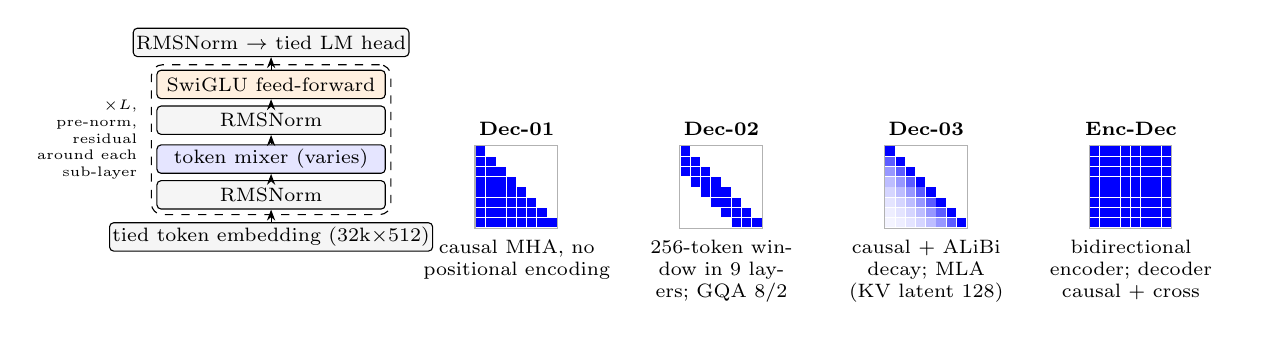
\begin{tikzpicture}[font=\scriptsize, >={Stealth[length=1.4mm]},
  blk/.style={draw, rounded corners=1.5pt, minimum width=2.9cm, minimum height=3.6mm, align=center, inner sep=1pt}]
\node[blk, fill=gray!8] (emb) at (0,0) {tied token embedding (32k$\times$512)};
\node[blk, fill=gray!8, above=1.6mm of emb] (n1) {RMSNorm};
\node[blk, fill=blue!10, above=0.8mm of n1] (att) {token mixer (varies)};
\node[blk, fill=gray!8, above=1.2mm of att] (n2) {RMSNorm};
\node[blk, fill=orange!12, above=0.8mm of n2] (ffn) {SwiGLU feed-forward};
\node[blk, fill=gray!8, above=1.6mm of ffn] (out) {RMSNorm $\to$ tied LM head};
\draw[->] (emb) -- (n1); \draw[->] (n1) -- (att); \draw[->] (att) -- (n2); \draw[->] (n2) -- (ffn); \draw[->] (ffn) -- (out);
\node[draw, dashed, rounded corners, fit=(n1)(ffn), inner sep=1.8pt] (rep) {};
\node[left=0.5mm of rep, align=right, font=\tiny] {$\times L$,\\ pre-norm,\\ residual\\ around each\\ sub-layer};
\newcommand{\maskpanel}[4]{%
\begin{scope}[shift={(#1,1.15)}]
\foreach \i in {0,...,7}{\foreach \j in {0,...,7}{
  \ifcase#3
    \pgfmathsetmacro{\v}{(\j<=\i)?100:0}\or
    \pgfmathsetmacro{\v}{((\j<=\i)&&(\i-\j<3))?100:0}\or
    \pgfmathsetmacro{\v}{(\j<=\i)?100*exp(-0.45*(\i-\j)):0}\or
    \pgfmathsetmacro{\v}{100}
  \fi
  \fill[blue!\v!white] (\j*0.13,-\i*0.13) rectangle ++(0.12,-0.12);
}}
\draw[gray!60] (-0.01,0.01) rectangle (1.04,-1.04);
\node[above] at (0.52,0.01) {#2};
\node[below, align=center, text width=2.4cm] at (0.52,-1.06) {#4};
\end{scope}}
\maskpanel{2.6}{\textbf{Dec-01}}{0}{causal MHA, no positional encoding}
\maskpanel{5.2}{\textbf{Dec-02}}{1}{256-token window in 9 layers; GQA 8/2}
\maskpanel{7.8}{\textbf{Dec-03}}{2}{causal + ALiBi decay; MLA (KV latent 128)}
\maskpanel{10.4}{\textbf{Enc-Dec}}{3}{bidirectional encoder; decoder causal + cross}
\end{tikzpicture}
\caption{Phase-1 architecture. All backbones share the pre-norm block on the left and differ in the token mixer. Each panel shows which keys (columns) a query (rows) may attend to; Dec-03 shading is the ALiBi weight, and the Dec-02 panel shows a local layer.}
\label{fig:arch}
\end{figure}

\textbf{Design story.} Dec-01 was meant to be a plain baseline with rotary embeddings~\cite{su2021roformer}. Porting it to Phase~2 weeks later revealed that the attention factory silently dropped the RoPE argument: Dec-01 had trained with \emph{no} positional encoding. It still learned word order, because a causal mask leaks position: token $t$ attends to exactly $t$ keys~\cite{kazemnejad2023nope}. I kept it as a NoPE decoder, whose causal mask can never be removed. It also trained in fp32 by accident, at 7.5k instead of about 18k tokens/s.

For the second model I wanted a change motivated by the data rather than by size. Most dependencies in a judgment are local, while a few are long-range (party names, the Act under discussion). Dec-02 therefore uses a 256-token sliding window in nine of twelve layers and full attention in layers 3, 7 and 11, in the spirit of Longformer~\cite{beltagy2020longformer}, with grouped-query attention~\cite{ainslie2023gqa} using two KV heads. Dec-03 changes both the position and the KV mechanism: ALiBi~\cite{press2022alibi} adds $-m_h(i-j)$ to each attention logit, which multiplies the softmax by an exponential decay over distance with a different horizon per head, and multi-head latent attention~\cite{deepseek2024v2} passes keys and values through a 128-dimensional latent, which is all the KV cache stores.

The encoder--decoder was meant to supply a bidirectional encoder. Its first version inherited a default that made the encoder causal, and its generation treated hidden states as logits (byte-level garbage). After fixing generation and resubmitting it, I trained v2 with a unit-tested bidirectional encoder, an added masked-LM loss on the encoder, and windows sized from the measured tokens per word (768/256 tokens instead of 512/128, which had truncated prompts).

\textbf{Objective, mixing and decoding.} The decoders minimize next-token cross-entropy on 1,024-token windows, with sources sampled in proportion to their token counts (13\% acts, 43\% High Courts, 17\% Supreme Court, 27\% tribunals). The consumed budgets differ sharply (Table~\ref{tab:arch}), which matters in Section~\ref{sec:results}. Every submission generates at least 128 words: the end token is masked until the word count is reached, repeated $n$-grams are banned, a repetition penalty of 1.1 is applied, the prompt is left-truncated so the most recent text is kept, and outputs are cut to exactly 128 words. The winning encoder--decoder submission is greedy.

\subsection{Transfer protocol (Phases 2--7)}
Every downstream model starts from a Phase-1 checkpoint (Fig.~\ref{fig:system}); none is trained from scratch. I implemented LoRA~\cite{hu2022lora}, LoRMA~\cite{bihany2025lorma} (compulsory), rsLoRA~\cite{kalajdzievski2023rslora}, IA$^3$~\cite{liu2022ia3}, Houlsby adapters~\cite{houlsby2019adapters}, prefix tuning~\cite{li2021prefix}, QLoRA~\cite{dettmers2023qlora} with my own NF4 quantizer, partial fine-tuning with layer-wise learning-rate decay~\cite{howard2018ulmfit}, full fine-tuning and knowledge distillation~\cite{hinton2015distilling}. Every adapter starts as the identity; an assertion checks that the adapted network reproduces the Phase-1 outputs exactly.

Two choices recur. First, a causally pretrained decoder can be \emph{unmasked} for understanding tasks: with RoPE or ALiBi it still knows positions, so removing the causal mask gives every token right context; for ALiBi I use the symmetric bias $-m_h|i-j|$. Dec-01 cannot be unmasked, so it either stays causal or reads its input twice and is pooled from the second copy (``echo''). Second, the distillation student is always Dec-03 with every second block kept (blocks $0,2,\dots,12$; 36.6M parameters), fully fine-tuned. It never loads the teacher's weights: the teacher writes its soft labels or scores to a file once, so it can be any architecture. The loss is
\begin{equation}
\mathcal{L} = \alpha\,T^2\,\mathrm{KL}\!\left(p_t^{(T)} \,\|\, p_s^{(T)}\right) + (1-\alpha)\,\mathcal{L}_\text{task},
\end{equation}
where $p^{(T)}$ are temperature-softened distributions; the $T^2$ factor keeps the soft term's gradient on the same scale as $T$ grows, which I verified against autograd.

\begin{figure}[t]
\centering
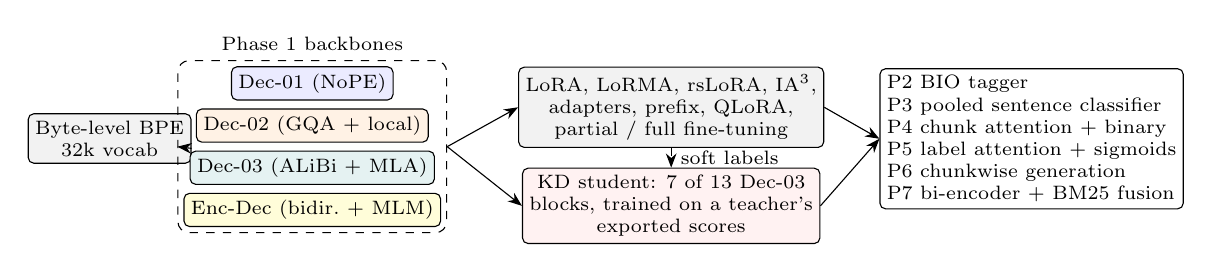
\begin{tikzpicture}[font=\scriptsize, node distance=2mm and 5mm,
  box/.style={draw, rounded corners=2pt, align=center, inner sep=2.5pt, fill=#1},
  box/.default=white, >={Stealth[length=1.8mm]}]
\node[box=gray!10] (tok) {Byte-level BPE\\32k vocab};
\node[box=blue!8, right=of tok, yshift=7mm] (d1) {Dec-01 (NoPE)};
\node[box=orange!10, below=1mm of d1] (d2) {Dec-02 (GQA + local)};
\node[box=teal!10, below=1mm of d2] (d3) {Dec-03 (ALiBi + MLA)};
\node[box=yellow!15, below=1mm of d3] (ed) {Enc-Dec (bidir.\ + MLM)};
\node[draw, dashed, rounded corners, fit=(d1)(d2)(d3)(ed), inner sep=2pt, label={[font=\scriptsize]above:Phase 1 backbones}] (bb) {};
\node[box=gray!10, right=9mm of bb, yshift=5mm] (ad) {LoRA, LoRMA, rsLoRA, IA$^3$,\\ adapters, prefix, QLoRA,\\ partial / full fine-tuning};
\node[box=pink!20, below=2.5mm of ad] (kd) {KD student: 7 of 13 Dec-03\\ blocks, trained on a teacher's\\ exported scores};
\node[box=white, right=7mm of ad, yshift=-4mm, align=left] (tasks) {P2 BIO tagger\\ P3 pooled sentence classifier\\ P4 chunk attention + binary\\ P5 label attention + sigmoids\\ P6 chunkwise generation\\ P7 bi-encoder + BM25 fusion};
\draw[->] (tok) -- (bb.west);
\draw[->] (bb.east) -- (ad.west);
\draw[->] (bb.east) -- (kd.west);
\draw[->] (ad.east) -- (tasks.west);
\draw[->] (kd.east) -- (tasks.west);
\draw[->, dashed] (ad.south) -- node[right, font=\scriptsize]{soft labels} (kd.north);
\end{tikzpicture}
\caption{System overview: one tokenizer, four Phase-1 backbones, and a separately fine-tuned descendant per phase and backbone. The student reads the teacher's predictions from a file, not its weights.}
\label{fig:system}
\end{figure}

\subsection{Phase 2 - Legal NER}
\vspace{-5pt}
NER is token classification with 25 BIO tags followed by span reconstruction through the stored offsets. Long documents are read in overlapping windows (800 tokens with stride 400 for decoders; 700/350 for the encoder, whose trained length is 768) and merged into one prediction per token. Class-weighted cross-entropy and a dev-tuned scale on the \texttt{O} logit handle imbalance. The winner is the Enc-Dec v2 encoder fully fine-tuned, which is the BERT recipe~\cite{devlin2019bert} on an encoder that was itself pretrained with a masked-LM loss.

\subsection{Phase 3 - Rhetorical role prediction}
\vspace{-5pt}
A window of consecutive sentences is encoded once; each sentence is the mean of its token states and is classified linearly, so one forward pass labels every sentence in the window with context from both sides. I train jointly on CL and IT with a short domain tag prepended to each window and select checkpoints on the mean of the two per-domain macro-F1 scores, so that the larger CL domain does not dominate.

\subsection{Phase 4 - Court judgment prediction}
\vspace{-5pt}
The last four 512-token chunks of a case are encoded and mean-pooled into $h_c$, and additive attention combines them, $\alpha_c=\mathrm{softmax}_c(w^\top\tanh(Wh_c))$, $d=\sum_c\alpha_c h_c$, before a logistic output. Because train is imbalanced (59/41) while dev is balanced, I tune the decision threshold on dev and keep it only if a two-fold check on dev confirms the gain; for the winner (Dec-01 with LoRA, $r=16$) it raised dev macro-F1 from 0.675 to 0.709.

\subsection{Phase 5 - Legal statute identification}
\vspace{-5pt}
Each statute has its own attention query over the token states of up to four 1,024-token chunks, followed by an independent sigmoid. The loss is binary cross-entropy with capped positive weights, and output biases start at the label priors so that training does not begin by predicting every statute. Thresholds are tuned on one half of dev and evaluated on the other, choosing between a global threshold, per-label thresholds, and per-label thresholds shrunk towards the global one in proportion to how few dev positives a label has. The winner is the distilled student.

\subsection{Phase 6 - Abstractive summarization}
\vspace{-5pt}
I aligned each reference sentence to its most similar source sentence and assigned it to the 512-token chunk containing that sentence; a chunk's target is its assigned sentences in summary order (at most 384 tokens for decoders and 255 for the encoder--decoder and student). Decoders read \texttt{[part $i$/$n$] chunk SUMMARY:} with loss on the target only; chunk summaries are concatenated in order. Length control was decisive (Section~\ref{sec:ablations}). The winning student used word-level KD on the teacher's token distributions plus sequence-level KD~\cite{kim2016seqkd}, i.e., the teacher's generated summaries as extra targets.

\subsection{Phase 7 - Prior Case Retrieval (PCR)}
\vspace{-5pt}
With exactly seven predictions per query, precision and recall share a numerator: for $H$ total hits, $N$ queries and $G$ gold pairs, $\text{F1@7}=2H/(7N+G)$, so the metric is the total number of hits. I first tuned BM25~\cite{robertson2009bm25}; the optimum ended at $k_1=8$, $b=1$ with uni- and bigrams. As $k_1\to\infty$ BM25 becomes length-normalized TF-IDF without saturation, which suits legal text where the thirtieth mention of a section is still evidence. The dense bi-encoder pools chunk vectors (mean, position-weighted mean~\cite{muennighoff2022sgpt} or last token), scores documents by cosine or MaxSim, and trains with multi-positive InfoNCE~\cite{oord2018cpc} ($\tau=0.05$) with one BM25 hard negative per pair and masking of other gold documents. Dense and BM25 scores are $z$-normalized and mixed with a dev-tuned weight, and each query is removed from its own pool. The winning student adds $0.7\cdot\mathrm{KL}$ between the teacher's and its own softmax over the BM25 top-300 list. A failed idea was the encoder's \texttt{[BOS]} vector as document embedding: 40--53 hits against 185--201 for mean pooling, since no pretraining loss ever asked that position to summarize its input.

% ============================================================
\section{Experiments and Implementation Details}
% ============================================================
\subsection{Compute and training protocol}
All runs used one Kaggle T4: four Phase-1 runs of 6.6--8.4 hours and 30 downstream runs of 1 minute to 3.6 hours. Sessions die after about nine hours, so every loop checkpoints every 20--25 minutes and resumes deterministically. All models use AdamW ($\beta=(0.9,0.95)$ in Phase~1, $(0.9,0.999)$ later), cosine decay after linear warmup, gradient clipping at 1.0, fp16 autocast with dynamic loss scaling (the T4 has no bf16), and no dropout; weight decay applies to two-dimensional weights only (a name-matching slip disabled it in Dec-01). Checkpoints are selected on a local dev metric: validation loss in Phases 1 and 6, macro-F1 in Phases 2--5 and dev hits@7 in Phase~7. Table~\ref{tab:hparams} lists each phase's winning configuration.

\begin{table}[t]
\centering
\footnotesize
\caption{Configuration of the winning model in each phase (P5--P7: the distilled student).}
\label{tab:hparams}
\setlength{\tabcolsep}{2.5pt}
\begin{tabular}{lccccccc}
\toprule
 & P1 & P2 & P3 & P4 & P5 & P6 & P7 \\
\midrule
Model & Enc-Dec & Encoder & Dec-03 & Dec-01 & Student & Student & Student \\
Method & pretrain & full FT & rsLoRA & LoRA & KD & KD & KD \\
Trainable params & 61.5M & 35.7M & 8.1M & 2.2M & 36.9M & 36.6M & 36.8M \\
Context (tokens) & 768/256 & 701 & 800 & $4\times512$ & $4\times1024$ & 512/255 & $\le16\times512$ \\
Peak LR & 6e-4 & 1e-4 & 5e-4 & 5e-4 & 2e-4 & 3e-4 & 1e-4 \\
Batch $\times$ accum. & $8\times8$ & 8 & 8 windows & $4\times4$ & 32 docs & 32 seqs & 16 queries \\
Epochs / steps & 15,488 steps & 5 ep. & 6 ep. & 4 ep. & 4 ep. & 4 ep. & 8 ep. \\
KD ($\alpha$, $T$) & -- & -- & -- & -- & 0.5, 2 & 0.5 + seq.\ KD & 0.7, 1 \\
Decoding / threshold & greedy & O-scale & argmax & tuned & shrunk & min.\ len. & fusion \\
\bottomrule
\end{tabular}
\end{table}

\subsection{Local evaluation}
\vspace{-5pt}
Test labels were never used: every choice (epoch, pooling, threshold, fusion weight, decoding) was made on local dev, and the Codabench score was recorded afterwards. A validator checked every zip's IDs, schema and phase rules before upload; it could not catch my one error, uploading a Phase-1 zip to Phase~2, so zips now carry their phase in the name. Local and test scores agree within 0.01 in Phases 2, 5, 6 and 7, but not in Phase~3 (0.480 vs.\ 0.438; ten test documents) or Phase~4, where test (0.725) exceeds the untuned dev score (0.675) because the submission used the tuned threshold.

\subsection{Ablations and controlled comparisons}
\vspace{-5pt}
\label{sec:ablations}
\textbf{Decoding, weights fixed.} In Phase~6 the same Dec-02+LoRMA weights scored ROUGE-1 0.20 with plain greedy decoding and 0.59 when each chunk had to produce at least 64 tokens (Fig.~\ref{fig:failures}b). 79\% of chunk outputs had been empty: greedy decoding stops once the end token beats the most likely word, and legal text spreads probability thinly. \textbf{Quantization.} In Phase~7, Dec-01 with QLoRA and with full fine-tuning share backbone, data and objective; storing the frozen weights in NF4 (4.13 bits per weight, relative error 0.093) changed nothing measurable (302 vs.\ 303 dense hits, 402 fused hits each) while training 3.9\% of the parameters. \textbf{Teacher signal.} Single- and three-teacher distillation in Phase~7 differ only in the target: the averaged target was flatter (lower KL) but not better (296 vs.\ 299 dense hits), because the teachers were of unequal quality (2,093, 1,923 and 1,582 training hits) and averaging adds the weaker teachers' errors. \textbf{Unmasking.} Making the top four Dec-03 blocks bidirectional changed zero-shot retrieval from 217 to 219 hits, so unmasking an ALiBi model costs nothing at step~0. \textbf{Pooling.} Zero-shot, position-weighted mean $\ge$ mean $\gg$ last token for every causal backbone, and mean-centering helps all of them (+20 to +27 hits for last-token pooling), consistent with anisotropy~\cite{ethayarajh2019contextual}. The Phase-1 architecture comparison (confounded by token budget) and Enc-Dec v1$\to$v2 (three changes at once) are \emph{not} clean, so I do not treat them as ablations.

% ============================================================
\section{Results}
\label{sec:results}
% ============================================================
\vspace{-5pt}
\begin{figure}[t]
\centering
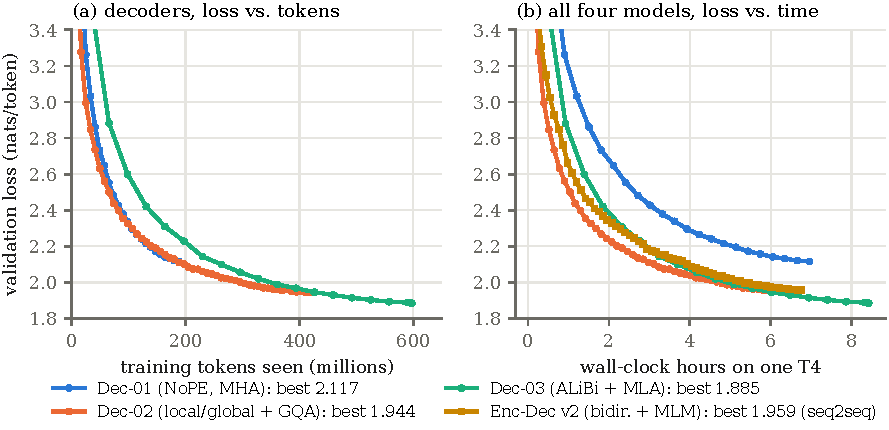
\includegraphics[width=0.68\linewidth]{figures/fig_p1_curves.pdf}
\caption{Phase-1 validation loss. (a) Against tokens seen, Dec-01 and Dec-02 are indistinguishable, and Dec-03 trails both until about 400M tokens; its lower final loss comes from seeing more tokens. (b) Against wall-clock time, Dec-01 is slowest because it accidentally trained in fp32.}
\label{fig:p1}
\end{figure}

\textbf{Phase 1.} Figure~\ref{fig:p1} overturns the obvious reading of Table~\ref{tab:arch}. Dec-03 has the lowest validation loss, but per token it learns more slowly: with 131k tokens per optimizer step against 33k, it makes four times fewer updates for the same data. Dec-01 and Dec-02 use the same step size and their curves coincide, so sliding-window attention with GQA cost nothing in quality at an equal budget while reducing attention cost in nine of twelve layers. None of this predicted the leaderboard: the encoder--decoder beat all six decoder submissions (BERTScore 0.836). It was trained on exactly ``prompt $\to$ continuation'' and always produced 128 words, whereas every decoder submission contained short outputs (minimum 1--72 words), which all three metrics penalize.

\begin{table}[t]
\centering
\footnotesize
\caption{Downstream variants: primary metric on local dev and on Codabench test (``--'': not submitted). Bold: the submitted winner of each phase. P3 dev is the mean per-domain macro-F1, P5 dev is the held-out half, P6 is BERTScore, P7 dev is fused F1@7.}
\label{tab:variants}
\setlength{\tabcolsep}{3pt}
\begin{tabular}{@{}cllcc@{\hspace{8pt}}cllcc@{}}
\toprule
Ph. & Variant & Train. & Dev & Test & Ph. & Variant & Train. & Dev & Test \\
\midrule
2 & \textbf{Enc-Dec enc., full FT} & 35.7M & .365 & \textbf{.373} & 5 & \textbf{KD student} & 36.9M & .438 & \textbf{.440} \\
2 & Dec-01, LoRA (echo) & 1.9M & .321 & .331 & 5 & Dec-03, partial FT & 11.9M & .414 & .416 \\
2 & KD student & 36.6M & .315 & -- & 5 & Dec-02, LoRMA (teacher) & 2.3M & .410 & .405 \\
2 & Dec-03, partial FT & 11.6M & .294 & .328 & 5 & Dec-01, full FT & 55.3M & .408 & .406 \\
2 & Dec-02, LoRMA & 2.0M & .270 & .292 & 5 & Enc-Dec enc., adapters & 1.2M & .385 & .390 \\
\cmidrule(r{10pt}){1-5}\cmidrule{6-10}
3 & \textbf{Dec-03, rsLoRA} & 8.1M & .480 & \textbf{.438} & 6 & \textbf{KD student} & 36.6M & .854 & \textbf{.851} \\
3 & Dec-02, LoRMA & 2.0M & .478 & .402 & 6 & Enc-Dec, adapters (teacher) & 2.0M & .856 & .851 \\
3 & Dec-01, LoRA (echo) & 1.9M & .467 & .397 & 6 & Dec-02, LoRMA & 2.0M & .851 & .848 \\
3 & Enc-Dec enc., IA$^3$ & 0.02M & .402 & .419 & 6 & Dec-01, prefix tuning & 1.7M & .842 & .839 \\
\cmidrule(r{10pt}){1-5}\cmidrule{6-10}
4 & \textbf{Dec-01, LoRA} & 2.2M & .675 & \textbf{.725} & 7 & \textbf{KD student, 1 teacher} & 36.8M & .448 & \textbf{.439} \\
4 & Enc-Dec enc., IA$^3$ & 0.28M & .644 & .632 & 7 & Enc-Dec enc., IA$^3$ & 0.28M & .445 & .437 \\
4 & KD student & 36.8M & .608 & .616 & 7 & Dec-01, full FT & 55.2M & .447 & .435 \\
4 & Dec-02, LoRMA (teacher) & 2.2M & .542 & .606 & 7 & Dec-02, LoRMA (teacher) & 2.2M & .450 & .435 \\
4 & Dec-03, rsLoRA (diverged) & 8.4M & .364 & .526 & 7 & Dec-03, partial FT & 11.8M & .448 & -- \\
 & & & & & 7 & Dec-01, QLoRA & 2.2M & .447 & .434 \\
 & & & & & 7 & KD student, 3 teachers & 36.8M & .446 & .432 \\
 & & & & & 7 & BM25 only & -- & .439 & .431 \\
\bottomrule
\end{tabular}
\end{table}

\begin{figure}[t]
\centering
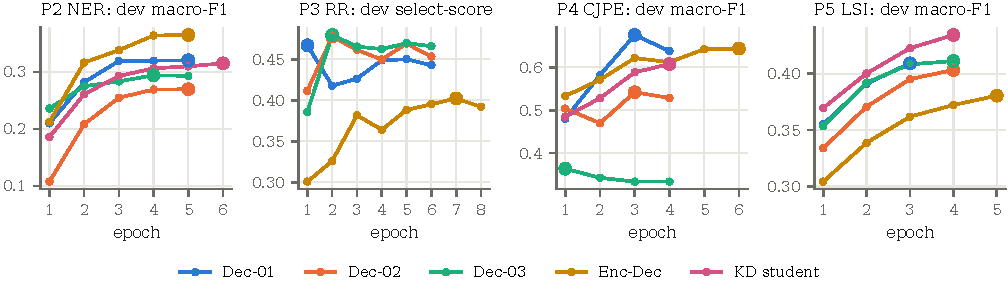
\includegraphics[width=0.92\linewidth]{figures/fig_epochs.pdf}
\caption{Dev metric after each epoch for every Phase 2--5 run; circles mark the selected checkpoint. Phase~3 peaks after one or two epochs and then overfits; Phase~5 is still improving at the last epoch; Dec-03 in Phase~4 never leaves chance.}
\label{fig:epochs}
\end{figure}

\textbf{Phases 2--7.} Table~\ref{tab:variants} lists every downstream variant and Fig.~\ref{fig:epochs} their dev curves. The bidirectional encoder did best where each token needs context from both sides (NER: 0.365 against at most 0.321 for decoders). Adapting a few million parameters is usually enough: full fine-tuning won only Phase~2, and in Phase~7 every method from 0.28M to 55M trainable parameters reached about 300 dense hits (Fig.~\ref{fig:kd}b). Distillation was the most reliable method (Fig.~\ref{fig:kd}a). The student (36.6--36.9M) came within 2\% of its teacher (56.8--63.5M) in Phases 2, 6 and 7, and beat it in Phases~4 (0.608 vs.\ 0.542) and 5 (0.438 vs.\ 0.410 held-out), on test as well (0.616 vs.\ 0.606; 0.440 vs.\ 0.405). Both times the teacher was Dec-02 with LoRMA on a frozen network. The student uses the soft labels as a regularizer but has full capacity of its own, so it can fit the task better than the adapter that taught it; in Phase~5 the soft labels also encode which statutes co-occur, which a one-hot target does not. On test the student won Phases 5, 6 and 7, but the Phase-6 and Phase-7 margins (0.854 vs.\ 0.856 on dev; 0.439 vs.\ 0.437 on test) are within noise, so I read them as ties; in Phase~6 the student does this with 42\% fewer parameters than its 63.5M teacher.

\begin{figure}[t]
\centering
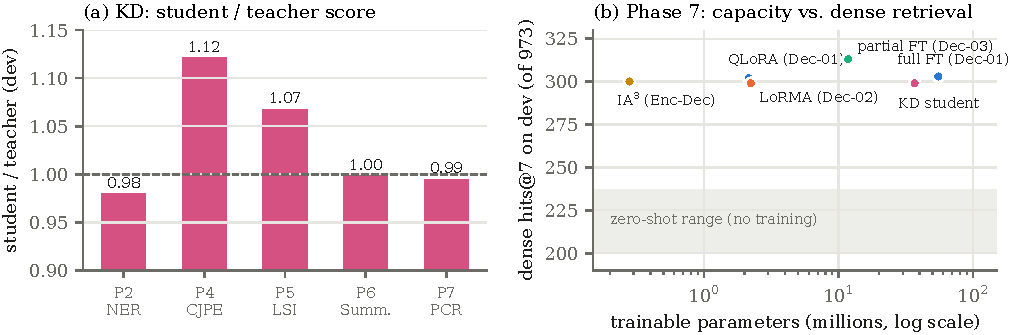
\includegraphics[width=0.64\linewidth]{figures/fig_kd_capacity.pdf}
\caption{(a) Student score divided by teacher score on local dev (student 36.6--36.9M parameters, teachers 56.8--63.5M). (b) Phase-7 dense retrieval against trainable parameters: a 200-fold range of capacity gives the same result, so the 827 training queries, not capacity, limit learning.}
\label{fig:kd}
\end{figure}

% ============================================================
\section{Error Analysis and Discussion}
% ============================================================
\vspace{-5pt}
\subsection{Phase-wise failure modes}
\vspace{-5pt}
\textbf{Phase 1.} 40 of Dec-01's and 58 of Dec-03's continuations stop before 128 words, mostly after a learned end-of-document token, and fluent outputs drift into generic procedural prose that keeps BERTScore high but ROUGE-L below 0.2.

\textbf{Phase 2.} Figure~\ref{fig:data}b shows the cleanest pattern in the project. Entities defined by form are learned (DATE 0.89, COURT 0.78, STAT 0.69); entities defined by their role in the case are not (APP 0.04, RESP 0.06, with 370 and 348 predicted spans of which 12 and 15 are correct). The model finds party names but not which side they are on, which is settled by words like ``appellant'' that may be hundreds of tokens away. It is not a frequency problem: APP has three times the training examples of JUDGE (0.42).

\textbf{Phase 3.} CL is harder than IT for every model (0.47 vs.\ 0.49 for the winner), and near-absent labels such as \emph{Issue} (17 CL training sentences) cost $1/13$ of macro-F1 when missed. Separating lower-court from present-court rulings requires knowing which court is speaking, often outside an 800-token window.

\textbf{Phase 4 (a failed run).} Dec-03 with rsLoRA never learned. Its training loss stayed at $\ln 2$, the loss of always predicting 0.5, for 5,200 steps and then became NaN (Fig.~\ref{fig:failures}a); the submission used the epoch-1 checkpoint. With $r=64$, $\gamma=\alpha/\sqrt{r}=2$ on every projection and learning rate $5\times10^{-4}$, the update was large, and on long fp16 chunks an activation eventually overflowed. The same method worked on Dec-03 in Phase~3, and a Dec-03-based student trained normally on this task, so the recipe failed, not the backbone.

\begin{figure}[t]
\centering
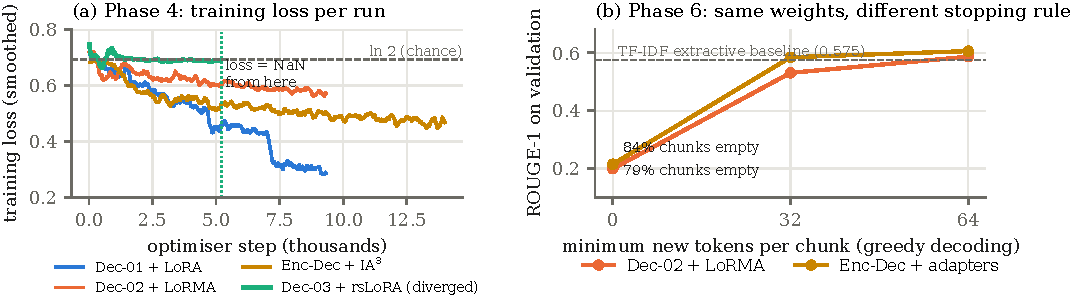
\includegraphics[width=0.62\linewidth]{figures/fig_p4_p6.pdf}
\caption{(a) Phase-4 training loss per run, smoothed over 200 steps: Dec-03 with rsLoRA stays at chance and then diverges. (b) Phase-6 ROUGE-1 as a function of the minimum number of tokens generated per chunk, with the trained weights held fixed.}
\label{fig:failures}
\end{figure}

\textbf{Phases 5--7.} The worst statutes have hundreds of training documents but F1 near 0.1 (statute~8: 349, F1 0.09): confusable neighbours, not rarity. Short Phase-5 documents score far lower (0.31 vs.\ 0.42), as a 225-token order states few facts. In Phase~6 the encoder--decoder copies more than the references (novel 4-grams 0.38 vs.\ 0.48), and for documents over 8k tokens ROUGE-L drops from 0.34 to 0.28 as chunks are skipped. Dense retrieval adds only ten hits over BM25 (405 vs.\ 395).

\subsection{What the metrics do not measure}
\vspace{-5pt}
BERTScore and ROUGE reward similarity to one reference, not legal correctness: a summary can omit the holding at little cost. Span-F1 scores a boundary slip and a wrong party role identically, and F1@7 weighs every citation equally. Those are the errors that matter most in practice, so a lawyer would still have to check party roles, holdings and precedents by hand.

\subsection{Limitations and what you would do next}
\vspace{-5pt}
Pretraining budgets were small and unequal, and the Phase-3 distillation run was never completed. Next I would (i) retrain all decoders, Dec-01 with RoPE, at an equal 600M-token budget; (ii) resolve party roles from the case title; (iii) rerun Dec-03+rsLoRA with $\alpha=8$ and fp32 attention logits; and (iv) run a KD control with $\alpha=0$ to isolate the soft labels' effect.

\subsection{Surprising findings}
\vspace{-5pt}
The lowest-loss model (Dec-03) did not win Phase~1; a student with 64\% of its teacher's parameters (36.8M vs.\ 57.2M, Phase~4) beat the teacher twice; and 0.28M and 55M trainable parameters retrieved the same number of hits.

% ============================================================
\section{Conclusion}
% ============================================================
\vspace{-5pt}
Across the seven phases, how a model was trained and used mattered more than which attention variant it had. In Phase~1 the encoder--decoder won not because it had the lowest loss but because it was trained on exactly the task and always wrote 128 words. Bidirectional context decided NER in Phase~2, a few million adapted parameters were enough for rhetorical roles and judgment prediction in Phases 3 and 4, and distillation into a fully trainable student gave the best or joint-best result in statute identification, summarization and retrieval in Phases 5 to 7. The largest single gain came from decoding rather than training: forcing a minimum output length nearly tripled Phase-6 ROUGE-1 with the same weights. What still fails is reasoning over the whole document, such as working out who the appellant is or which court is speaking, and that is where I would spend the next compute budget.

% ============================================================
\section*{LLM Usage Declaration}
% ============================================================
Completing this section is mandatory. Inconsistent answers relative to the code and the prose will be treated as an integrity issue.
\medskip

\noindent
\textbf{Q1.} Which Large Language Model(s), if any, did you use while completing the competition or writing this report? Give model name and vendor (e.g., none / ChatGPT-4.x / Gemini~x / Claude~x / Grok / Copilot / other). \\[0.6em]
Answer: Gemini 3.1 Pro, Claude Sonnet 5.5

\medskip
\noindent
\textbf{Q2.} For each row, mark Yes or No and state the purpose in one short phrase.
\begin{table}[H]
\centering
\begin{tabular}{>{\raggedright\arraybackslash}p{4.6cm}|c|>{\raggedright\arraybackslash}p{7.2cm}}
\toprule
Part & Used LLM? & Purpose of using the LLM \\
\midrule
Understanding concepts / papers & Yes &  Help with understanding all the concepts involved across the projects \\
Ideation / brainstorming at a high level & Yes & Help with my ideas, if they are good enough to be explored more, or outright bad to be dropped instantly and move on \\
Debugging small ancillary snippets & Yes & Help with little areas of code here and there \\
Plotting / visualization code & Yes & Help write the code for plotting and visualizing the figures of the report and notebooks \\
Grammar / writing style of the report & Yes & Check for any grammatical mistakes \\
Report structure / section wording & No &  LLM not used \\
Designing the model architecture & No & LLM not used \\
Hyperparameter search / tuning & No &  LLM not used \\
Analysis of results / conclusions & No & LLM not used \\
Writing the core training / inference code & No &  LLM not used \\
Other (specify) & Yes & Used LLM to go through the papers listed in the bibliography. Used LLM to generate the references for all the concepts I used throughout the project across notebooks \\
\bottomrule
\end{tabular}
\end{table}

\medskip
\noindent
\textbf{Q3.} Did you refer to sources other than lecture slides and an LLM?
If yes, list them (papers, blogs, GitHub repositories, textbooks, official starter notebook, evaluation scripts). These must also appear in the bibliography when they influenced the method. \\[0.4em]
Answer:
Yes. Papers listed in the bibliography (consulted mainly through the LLM and lecture material); the official \texttt{Exploration-Lab/CS-781-Capstone} dataset on Hugging Face; the \texttt{bert\_score} and \texttt{rouge\_score} Python packages for local evaluation.

\medskip
\noindent
\textbf{Q4.} Apart from any permitted LLM use, what was \emph{your} contribution? In 8--12 sentences describe your own understanding, architecture decisions, implementation, experiments, and analysis. Name at least two things you tried that failed and what you concluded from them. \\[0.4em]

Answer: I pretrained four small Transformer language models (54--63M parameters) from scratch on Indian legal text, using my own 32k byte-level BPE tokenizer and plain PyTorch, and then adapted them to six downstream legal tasks. Since most dependencies in a judgment are local and only a few (party names, statute references) are long-range, I built a plain causal baseline (Dec-01), a sliding-window decoder with grouped-query attention (Dec-02), an ALiBi decoder with multi-head latent attention (Dec-03), and an encoder--decoder whose bidirectional encoder was also trained with a masked-LM loss. For the downstream phases I implemented LoRA, LoRMA, rsLoRA, IA\textsuperscript{3}, adapters, prefix tuning, QLoRA with my own NF4 quantizer, partial and full fine-tuning, and distillation into a 7-block Dec-03 student, with every choice made on local dev and every zip checked by a validator before upload. The bidirectional encoder won Phase 1 and the NER phase, and the distilled student won Phases 5--7 and twice beat its larger Dec-02 teacher. Adapting a few million parameters was usually enough; in retrieval, 0.28M and 55M trainable parameters gave the same number of hits. Several things failed. A bug silently dropped RoPE from Dec-01, so it trained with no positional encoding; it still learned word order from the causal mask, but for that reason it could never be unmasked for the understanding tasks. Dec-03 with rsLoRA diverged in Phase 4 (loss stuck at $\ln 2$, then NaN), but the same method worked in Phase 3 and a Dec-03 student trained normally on this task, so I concluded that the recipe failed, not the backbone. In summarization, 79\% of greedy chunk outputs were empty, and forcing a minimum length raised ROUGE-1 from 0.20 to 0.59 with the same weights, which showed that decoding mattered more than training there. Distilling from three teachers instead of one did not help, because averaging added the weaker teachers' errors. Finally, Dec-03's lower validation loss came from seeing three times more tokens, not from a better architecture, and the remaining errors, such as telling appellant from respondent, need reasoning over the whole document, which a 55M model reading 1,024 tokens at a time cannot do.


\bibliographystyle{ieeetr}
\bibliography{references_report}
\end{document}
